\documentclass[a4paper, 14pt]{extarticle}
\usepackage{enumitem}
\usepackage{fefutitle}
\usepackage{listings}
\usepackage{xcolor}
\usepackage{amsmath}
\usepackage{graphicx}
\usepackage[justification=centering]{caption}
\usepackage{float}

\lstdefinestyle{mystyle}{
	basicstyle={\small\ttfamily},
	keywordstyle=\color{orange},
	stringstyle=\color{green},
	basicstyle=\ttfamily\footnotesize,
	breakatwhitespace=false,         
	breaklines=true,                 
	captionpos=b,                    
	keepspaces=true,                 
	numbers=none,                    
	numbersep=5pt,                  
	showspaces=false,                
	showstringspaces=false,
	showtabs=false,                  
	tabsize=2,
	aboveskip=3mm,
	belowskip=3mm,
}
\lstset{style=mystyle}

\begin{document}
	\fefutitle{2}
	\pagebreak	

	\section{Определение цели}
		В данной лабораторной необходимо создать модель электрического утюга с терморегулятором и без него.
		Проанализировать полученную модуль.

	\section{Информация об объекте}
		Утюг - нагревающийся металлический прибор. Работа утюга с электрическим нагревом основана на выделении тепловой энергии при прохождении электрического тока через нагревательный элемент. Температура нагревательного элемента сообщается подошве утюга, которая также нагревается.
		
		Температура нагрева задается отдельным терморегулятором, главная функция которого заключается в своевременном отключении подачи электроэнергии в соответствии с заданным режимом.

	\section{Создание математической модели}
		Введем характеристики, которые необходимы для создания модели:
		\begin{enumerate}[leftmargin=3\parindent, itemsep=0mm]
			\item m - масса подошвы утюга
			\item c - удельная теплоёмкость подошвы утюга
			\item S - площать поверхности подошвы
			\item P - электрическая мощность утюга
			\item T - температура утюга
			\item $T_a = 293K = 20^{\circ}C$ - температура окружающей среды
		\end{enumerate}
	
		Количество теплоты(\(\Delta Q\)), которое получает тело при увеличении его температуры на величину 
		\( \Delta T = T_2 - T_1 \) вычисляется так:
		\[ \Delta Q = cm \Delta T \], где \( T_1, T_2\) - температуры тела до нагрева и после.
		
		Количество теплоты, отдаваемое утюгом в окружающую среду вычисляется по закону Ньютона-Рихмана:
		\[ Q = kS(T-T_a) \Delta t \]
		, где \(k\) - коэффициент теплообмена
			
		Нагретые тела излучают энергию в виде электромагнитных волн различной длины. Тепловое излучение:
		\[ E = \sigma T^4 \]
		, где \( \sigma = 5.67 \cdot 10^{-8} \) - постоянная Стефана-Больцмана
		
		Составим уравнение теплового баланса:
		\[ \Delta Q = P\Delta t - kS(T-T_a) \Delta t - S \sigma T^4 \Delta t +  S \sigma T_a^4 \Delta t\]
		\[ cm \Delta T = P\Delta t - kS(T-T_a) \Delta t - S \sigma (T^4 - T_a) \Delta t \]
		
		Поделим на \( \Delta t\) и умножим на \(cm\)
		\[ \dfrac{\Delta T}{\Delta t} 
		= \dfrac{P - kS(T-T_a) - S \sigma T^4 +  S \sigma T_a^4}{cm}\]
		
		Перейдём к дифференциальному уравнению и добавим начальное условие(в начальный момент времени
		температура подошвы утюга равна температуре окружающей среды):
		\[
			\begin{cases}
				\dfrac{\Delta T}{\Delta t} = \dfrac{P - kS(T-T_a) - S \sigma (T^4 - T_a) \Delta t}{cm},\\
				T(0) = T_a.
			\end{cases}
		\]
		
		Для утюга с терморегулятором добавим функцию, которая будет отвечать за включение и отключение утюга
		после достижения заданной максимальной температуры $T_{max}$
		\[ H(T) = 
			\begin{cases}
				0, \text{если} T >= T_{max}\\
				1, \text{если} T <= T_{min}
			\end{cases} 
		\]
		
		Тогда дифференциальное уравнение примет следующий вид:
		\[
		\begin{cases}
			\dfrac{\Delta T}{\Delta t} = \dfrac{ P\cdot H(T) - kS(T-T_a) - S \sigma (T^4 - T_a) \Delta t}{cm},\\
			T(0) = T_a.
		\end{cases}
		\]
	
	\section{Анализ модели}
		\setlength\parindent{0pt}
		Программы были написаны на языке Java.
		\subsection{Утюг без терморегулятора}
			Код программы:
			\begin{lstlisting}[language=Java]
public class Main {
	private static final Integer T0 = 291;
	private static Integer state = HEATING;
	
	private static class Func implements Function<Double, Double> {
		@Override
		public Double apply(Double T) {
			double sigma = 5.67E-8;
			int P = 1600;
			int c = 900;
			double m = 0.8;
			double s = 0.02;
			int k = 25;
			return (P - k * s *(T - T0) - s * sigma *(Math.pow(T, 4) - Math.pow(T0, 4))) / c * m;
		}
	}
	
	private static ArrayList<Double> euler(Function<Double, Double> func, ArrayList<Integer> t) {
		ArrayList<Double> res = new ArrayList<>();
		
		double T = T0.doubleValue();
		for (int tValue: t) {
			T += func.apply(T);
			res.add(T);
		}
		return res;
	}
	
	public static void main(String[] args) throws PythonExecutionException, IOException {
		ArrayList<Integer> t = new ArrayList<>();
		for(int i = 0; i <= 1000; ++i) {
			t.add(i);
		}
		
		ArrayList<Double> T = euler(new Func(), t);
		
		Plot plt = Plot.create();
		plt.plot().add(t, T);
		plt.xlabel("t");
		plt.ylabel("T");
		plt.show();
	}
}
			\end{lstlisting}
			$P = 1600$ Вт
			
			$m = 0.8$ кг
			
			$c = 900$ Дж/К(Темплоёмкость алюминия)
			
			$S = 0.02 \text{м}^2$
			
			\begin{figure}[H]
				\centering
				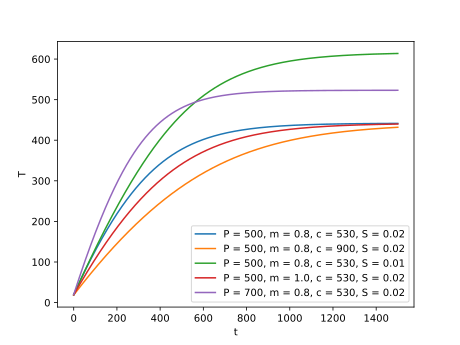
\includegraphics[width = \linewidth]{fig1.pdf}
				\caption[.] {}
			\end{figure}
			\pagebreak
		
			$P = 1600$ Вт
			
			$m = 0.8$ кг
			
			$c = 530$ Дж/К(Темплоёмкость титана)
			
			$S = 0.02 \text{м}^2$
			
			\begin{figure}[H]
				\centering
				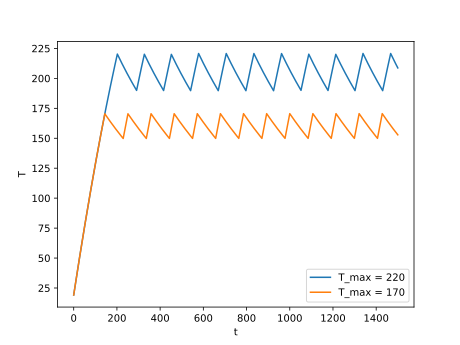
\includegraphics[width = \linewidth]{fig2.pdf}
				\caption[.] {}
			\end{figure}
			При использовании материала с меньшей теплоёмкостью скорость нагрева увеличивается.
			\pagebreak
			
			$P = 1600$ Вт
			
			$m = 1.2$ кг
			
			$c = 900$ Дж/К(Темплоёмкость алюминия)
			
			$S = 0.02 \text{м}^2$
			
			\begin{figure}[H]
				\centering
				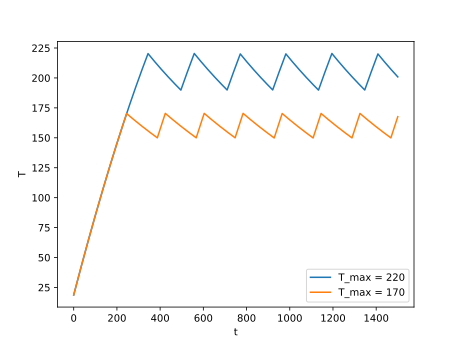
\includegraphics[width = \linewidth]{fig3.pdf}
				\caption[.] {}
			\end{figure}
			При увеличении массы подошвы скорость нагрева уменьшается.
			\pagebreak
			
			$P = 1600$ Вт
			
			$m = 0.8$ кг
			
			$c = 900$ Дж/К(Темплоёмкость алюминия)
			
			$S = 0.01 \text{м}^2$
			
			\begin{figure}[H]
				\centering
				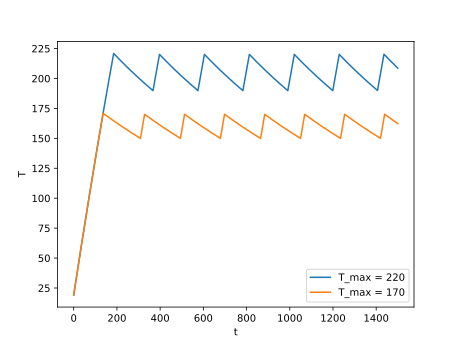
\includegraphics[width = \linewidth]{fig4.pdf}
				\caption[.] {}
			\end{figure}
			При уменьшении площади подошвы максимальная температура увеличивается.
			\pagebreak
			
			$P = 2000$ Вт
			
			$m = 0.8$ кг
			
			$c = 900$ Дж/К(Темплоёмкость алюминия)
			
			$S = 0.02 \text{м}^2$
			
			\begin{figure}[H]
				\centering
				\includegraphics[width = \linewidth]{fig10.pdf}
				\caption[.] {}
			\end{figure}
			При увеличении мощности увеличивается максимальная температура и скорость нагрева.
		\pagebreak
		\subsection{Утюг с терморегулятором}
			Код программы:
			\begin{lstlisting}[language=Java]
public class Main {
	private static final Integer COOLING = 0;
	private static final Integer HEATING = 1;
	private static final Integer T0 = 291;
	private static final Integer T_max = 483;
	private static final Integer T_min = 453;
	private static Integer state = HEATING;
	private static Integer thermostat(double T) {
		if (T >= T_max) {
			state = COOLING;
		} else if (T <= T_min) {
			state = HEATING;
		}
		return state.equals(COOLING) ? 0 : 1;
	}
	private static class Func implements Function<Double, Double> {
		@Override
		public Double apply(Double T) {
			double sigma = 5.67E-8;
			int P = 2000;
			int c = 900;
			double m = 0.8;
			double s = 0.02;
			int k = 25;
			return (P * thermostat(T)- k * s *(T - T0) - s * sigma *(Math.pow(T, 4) - Math.pow(T0, 4))) / (c * m);
		}
	}
	
	private static ArrayList<Double> euler(Function<Double, Double> func, ArrayList<Integer> t) {
		ArrayList<Double> res = new ArrayList<>();
		
		double T = T0.doubleValue();
		for (int tValue: t) {
			T += func.apply(T);
			res.add(T);
		}
		return res;
	}
	
	public static void main(String[] args) throws PythonExecutionException, IOException {
		ArrayList<Integer> t = new ArrayList<>();
		for(int i = 0; i <= 1500; ++i) {
			t.add(i);
		}
		
		ArrayList<Double> T = euler(new Func(), t);
		
		Plot plt = Plot.create();
		plt.plot().add(t, T);
		plt.xlabel("t");
		plt.ylabel("T");
		plt.savefig("fig10.svg");
		plt.show();
	}
				}
			\end{lstlisting}
			\pagebreak
			$P = 1600$ Вт
			
			$m = 0.8$ кг
			
			$c = 900$ Дж/К(Темплоёмкость алюминия)
			
			$S = 0.02 \text{м}^2$
			
			\begin{figure}[H]
				\centering
				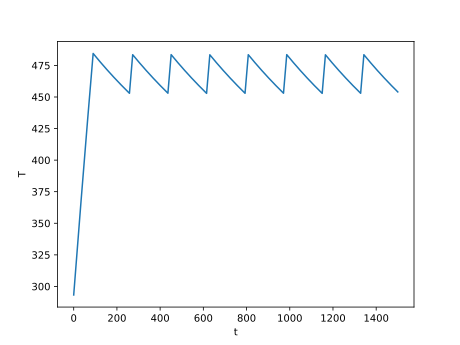
\includegraphics[width = \linewidth]{fig5.pdf}
				\caption[.] {}
			\end{figure}
			\pagebreak
			
			$P = 1600$ Вт
			
			$m = 0.8$ кг
			
			$c = 530$ Дж/К(Темплоёмкость титана)
			
			$S = 0.02 \text{м}^2$
			
			\begin{figure}[H]
				\centering
				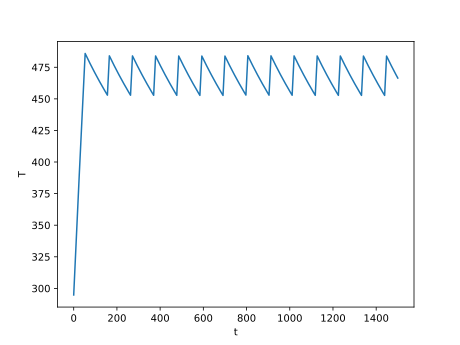
\includegraphics[width = \linewidth]{fig6.pdf}
				\caption[.] {}
			\end{figure}
			При использовании материала с меньшей теплоёмкостью колебания температур учащаются.
			\pagebreak
			
			$P = 1600$ Вт
			
			$m = 1.2$ кг
			
			$c = 900$ Дж/К(Темплоёмкость алюминия)
			
			$S = 0.02 \text{м}^2$
			
			\begin{figure}[H]
				\centering
				\includegraphics[width = \linewidth]{fig7.pdf}
				\caption[.] {}
			\end{figure}
			При увеличении массы подошвы скорость нагрева и частота колебаний температур уменьшаются.
			\pagebreak
			
			$P = 1600$ Вт
			
			$m = 0.8$ кг
			
			$c = 900$ Дж/К(Темплоёмкость алюминия)
			
			$S = 0.01 \text{м}^2$
			
			\begin{figure}[H]
				\centering
				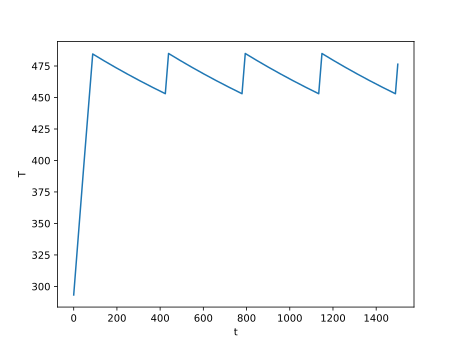
\includegraphics[width = \linewidth]{fig8.pdf}
				\caption[.] {}
			\end{figure}
			При уменьшении площади подошвы уменьшается частота колебаний температур.
			\pagebreak
			
			$P = 2000$ Вт
			
			$m = 0.8$ кг
			
			$c = 900$ Дж/К(Темплоёмкость алюминия)
			
			$S = 0.02 \text{м}^2$
			
			\begin{figure}[H]
				\centering
				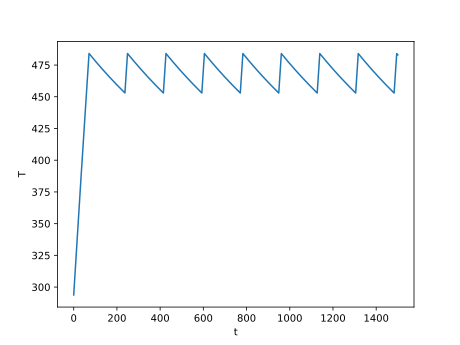
\includegraphics[width = \linewidth]{fig9.pdf}
				\caption[.] {}
			\end{figure}
			При увеличении мощности увеличиваются скорость нагрева и частота колебаний.
	\section{Вывод}
		Таким образом, построена математическая модель утюга с терморегулятором и без него. Она позволяет получить график температур от времени для утюгов с различными площадями подошвы, теплопроводностями и мощностями. 
		
\end{document}	